The PF reconstruction of isolated photons is conducted together with electron reconstruction.
This is because the large amount of material in the tracker makes electron emit bremsstrahlung photons, which may convert to \Pep \Pem pairs,
which may in turn produce bremsstrahlung, and so on.

Photon candidates are seeded by ECAL superclusters with $\ET > 10 \GeV$ with no link to a GSF track.
As for the electron candidates, the energy sum of the HCAL cells within $\DR = 0.15$ must not exceed 10 \% of the supercluster energy.
All ECAL clusters linked to the supercluster are associated with the candidate.

To correct for the energy missed in the association process,
a correction is applied to the total energy of the ECAL clusters with analytical functions of the energy and pseudorapidity, which can be as large as 25 \% at low \pt and maximum tracker thickness ($|\eta| \approx 1.5$).
The direction of the photon is taken to be that of the supercluster.

Photon candidates are retained if they are isolated from other tracks and calorimeter clusters in the event,
and if the ECAL cell energy distribution and the ratio between the HCAL and ECAL energies are compatible with those expected from a photon shower.
The PF selection is looser than the requirements applied at analysis level to select isolated photons.

\paragraph{Analysis selection for photons}
Photon candidates are reconstructed as Super-Clusters in the ECAL with $E_{T} > 20 GeV$ in the fiducial Barrel region and Endcap region, defined by $|\eta|<1.4442$ and $1.566<|\eta|<2.5$, respectively.
They are required to satisfy the loose cut-based selection \cite{CMS:EGM-17-001} seen in Table \ref{tab:VPhotonID}, which provides $90\%$ signal selection efficiency:

\begin{table}[h!]
\begin{center}
\scalebox{0.75}{
\begin{tabular}{|c|c|c|}
\hline 
\hline 
Requirement &  Barrel$\quad$$|\eta|<$1.4442 & Endcap$\quad$ 1.566$<|\eta|<$2.5 \\
\hline
%% Medium WP
%% $H/E<$ & 0.02197 & 0.0326 \\
%% $\sigma_{i\eta i\eta}<$ & 0.01015 & 0.0272 \\
%% Rho corrected PF charged hadron isolation $<$ & 1.141\ GeV & 1.051\ GeV\\
%% Rho corrected PF neutral hadron isolation$<$ & $1.189 + 0.01512*p_{T}^{\gamma} + 2.259e-05*p_{T}^{\gamma 2}$ & $2.718 + 0.0117*p_{T}^{\gamma} + 2.3e-05*p_{T}^{\gamma 2}$\\
%% Rho corrected PF photon isolation$<$ &$2.08 + 0.004017*p_{T}^{\gamma}$ & $3.867 + 0.0037*p_{T}^{\gamma}$\\
%% 
%% Loose WP
$H/E<$ & 0.04596 & 0.0590 \\
$\sigma_{i\eta i\eta}<$ & 0.0106 & 0.0272 \\
Rho corrected PF charged hadron isolation $<$ & 1.694\ GeV & 2.089\ GeV\\
Rho corrected PF neutral hadron isolation$<$ & $24.032 + 0.01512\, p_{T}^{\gamma} + 2.259 \cdot 10^{-5}\, p_{T}^{\gamma 2}$ & $19.722 + 0.0117\, p_{T}^{\gamma} + 2.3 \cdot 10^{-5}\, p_{T}^{\gamma 2}$\\
Rho corrected PF photon isolation$<$ & $2.876 + 0.004017\, p_{T}^{\gamma}$ & $4.162 + 0.0037\, p_{T}^{\gamma}$\\
Pass Conversion safe electron veto & True & True\\
\hline
\end{tabular}}
\caption[.]{Cut-based Loose photon ID for 94X and later samples}
\label{tab:VPhotonID}
\end{center}
\end{table}

%Barrel:
%
%\begin{itemize}
%\item Single tower H/E $<$ 0.0396 
%\item $\sigma_{i\eta i\eta}<0.01022$ 
%\item pile-up corrected PF charged hadron isolation $<$ 0.441, which charged hadrons originated from the hard interaction primary vertex.
%\item pile-up corrected PF neutral hadron isolation $< 2.725 + 0.0148*p_{T}^{\gamma} + 0.000017*p_{T}^{\gamma 2}$ 
%\item pile-up corrected PF photon isolation $<2.571 + 0.0047*p_{T}^{\gamma}$
%\item Conversion safe electron veto
%\end{itemize}
%
%Endcap:
%
%\begin{itemize}
%\item Single tower H/E $<$ 0.0219
%\item $\sigma_{i\eta i\eta}<0.03001$
%\item pile-up corrected PF charged hadron isolation $<$ 0.442, which charged hadrons originated from the hard interaction primary vertex.
%\item pile-up corrected PF neutral hadron isolation $< 1.715 + 0.0163*p_{T}^{\gamma} + 0.000014*p_{T}^{\gamma 2}$
%\item pile-up corrected PF photon isolation $<3.863 + 0.0034*p_{T}^{\gamma}$
%\item Conversion safe electron veto
%\end{itemize}

Isolation is performed for a cone of radius 0.3.
Pile-up corrected PF isolation is calculated using effective area corrections.
The photon candidates are also required to be separated from the lepton by at least $0.07$ in $\eta-\phi$ space, which highly reduces the contribution from FSR.
The same separation requirement is imposed between the photon candidates and the jets.

\subsubsection{Photon Identification}
\label{sec:photonID}

Both a cut-based and a MVA-based ID are employed and compared in the analysis.\\
Each has its own advantages and disadvantages.
Due to its nature, the cut-based ID can be easily inverted by reversing only one or a few of its cuts.
On the other hand, MVA-based ID is more effective at discriminating between signal and background, providing a higher signal-to-noise ratio.

\paragraph{Cut-based ID}
The cut-based loose photon ID, described in ~\cite{CMS:EGM-17-001} and shown in table~\ref{tab:VPhotonID} is employed.
The corresponding ID scale factors, shown in Figure \ref{fig:phEffSF} are applied following the recommendations provided by the CMS experts on electrons and photons reconstruction.

\begin{figure}
\subfigure [2016preVFP ] {\resizebox{.5\textwidth}{!}{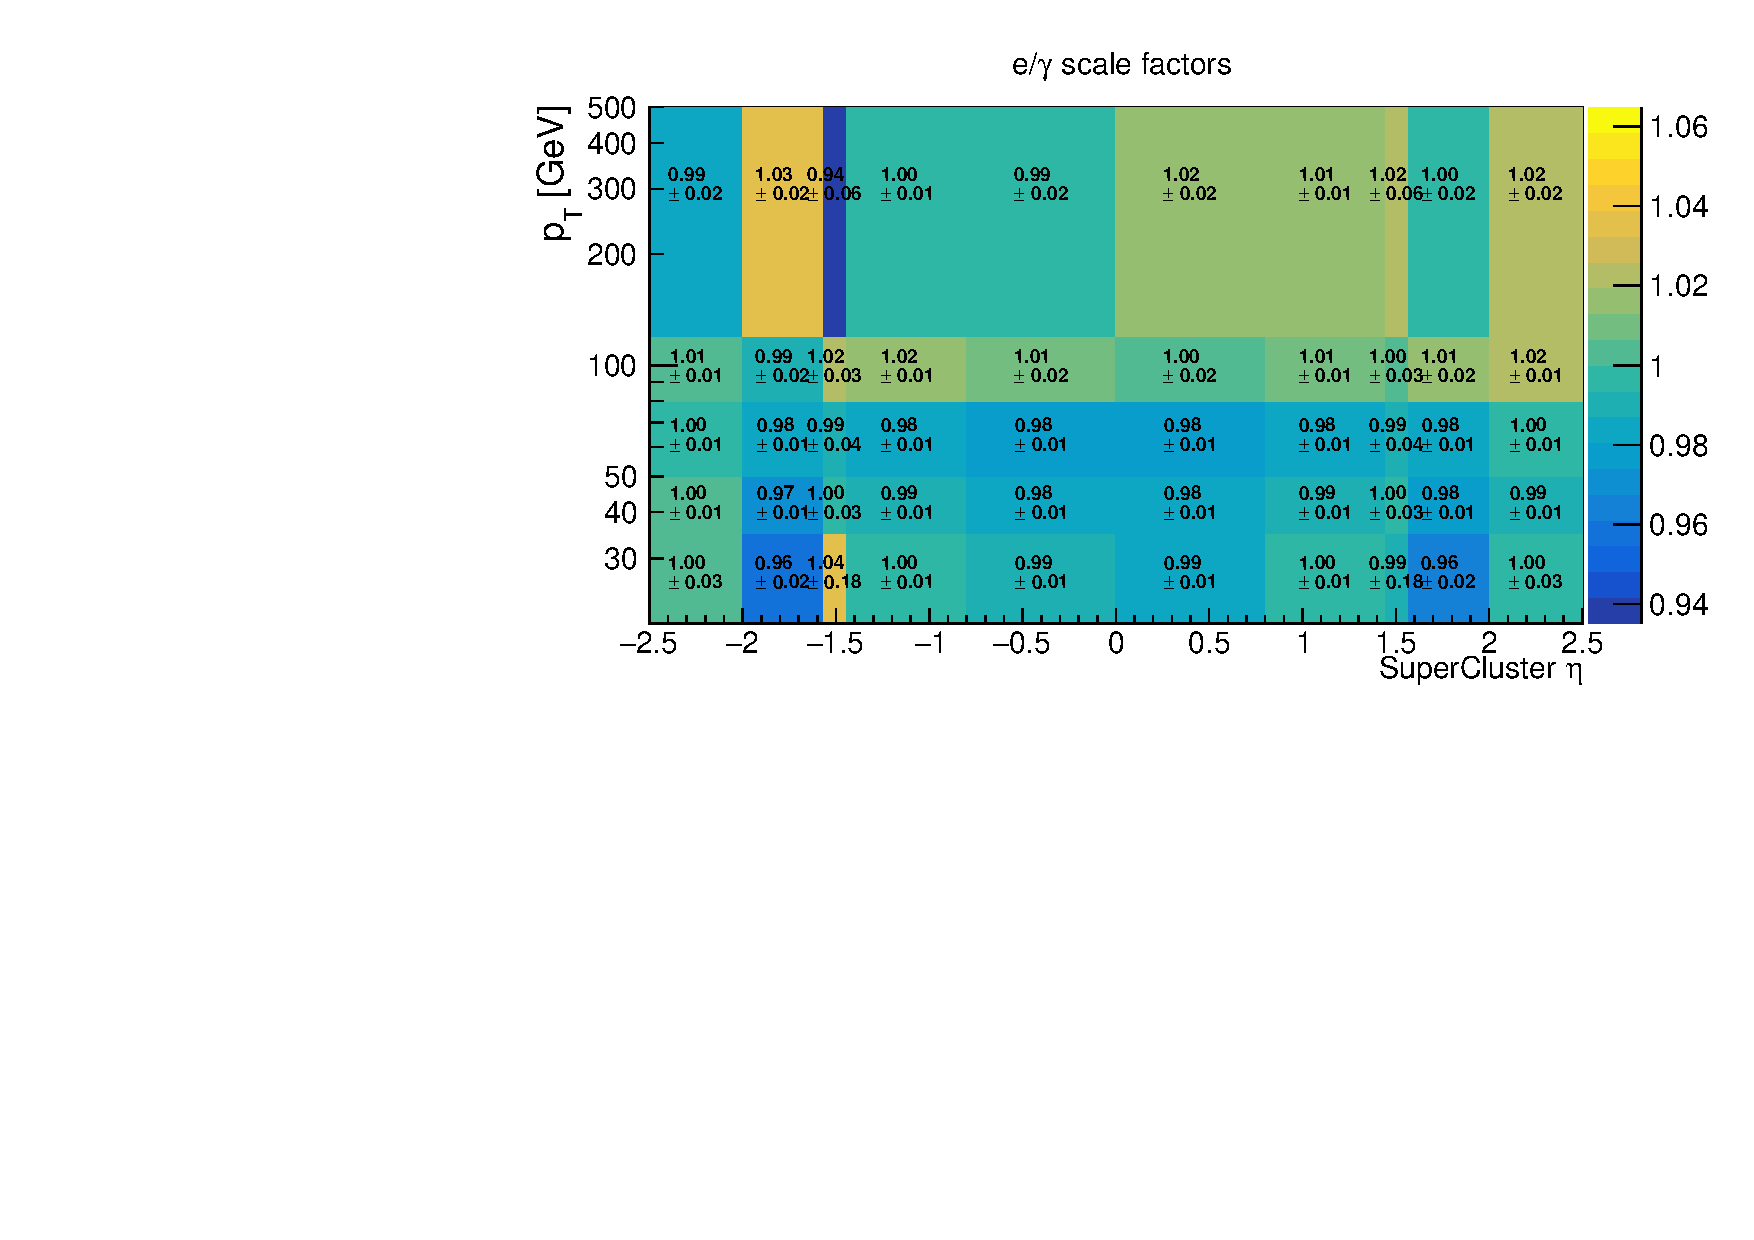
\includegraphics[width=.5\textwidth]{SF/phEffSF_2016preVFP.pdf} }}
\subfigure [2016postVFP] {\resizebox{.5\textwidth}{!}{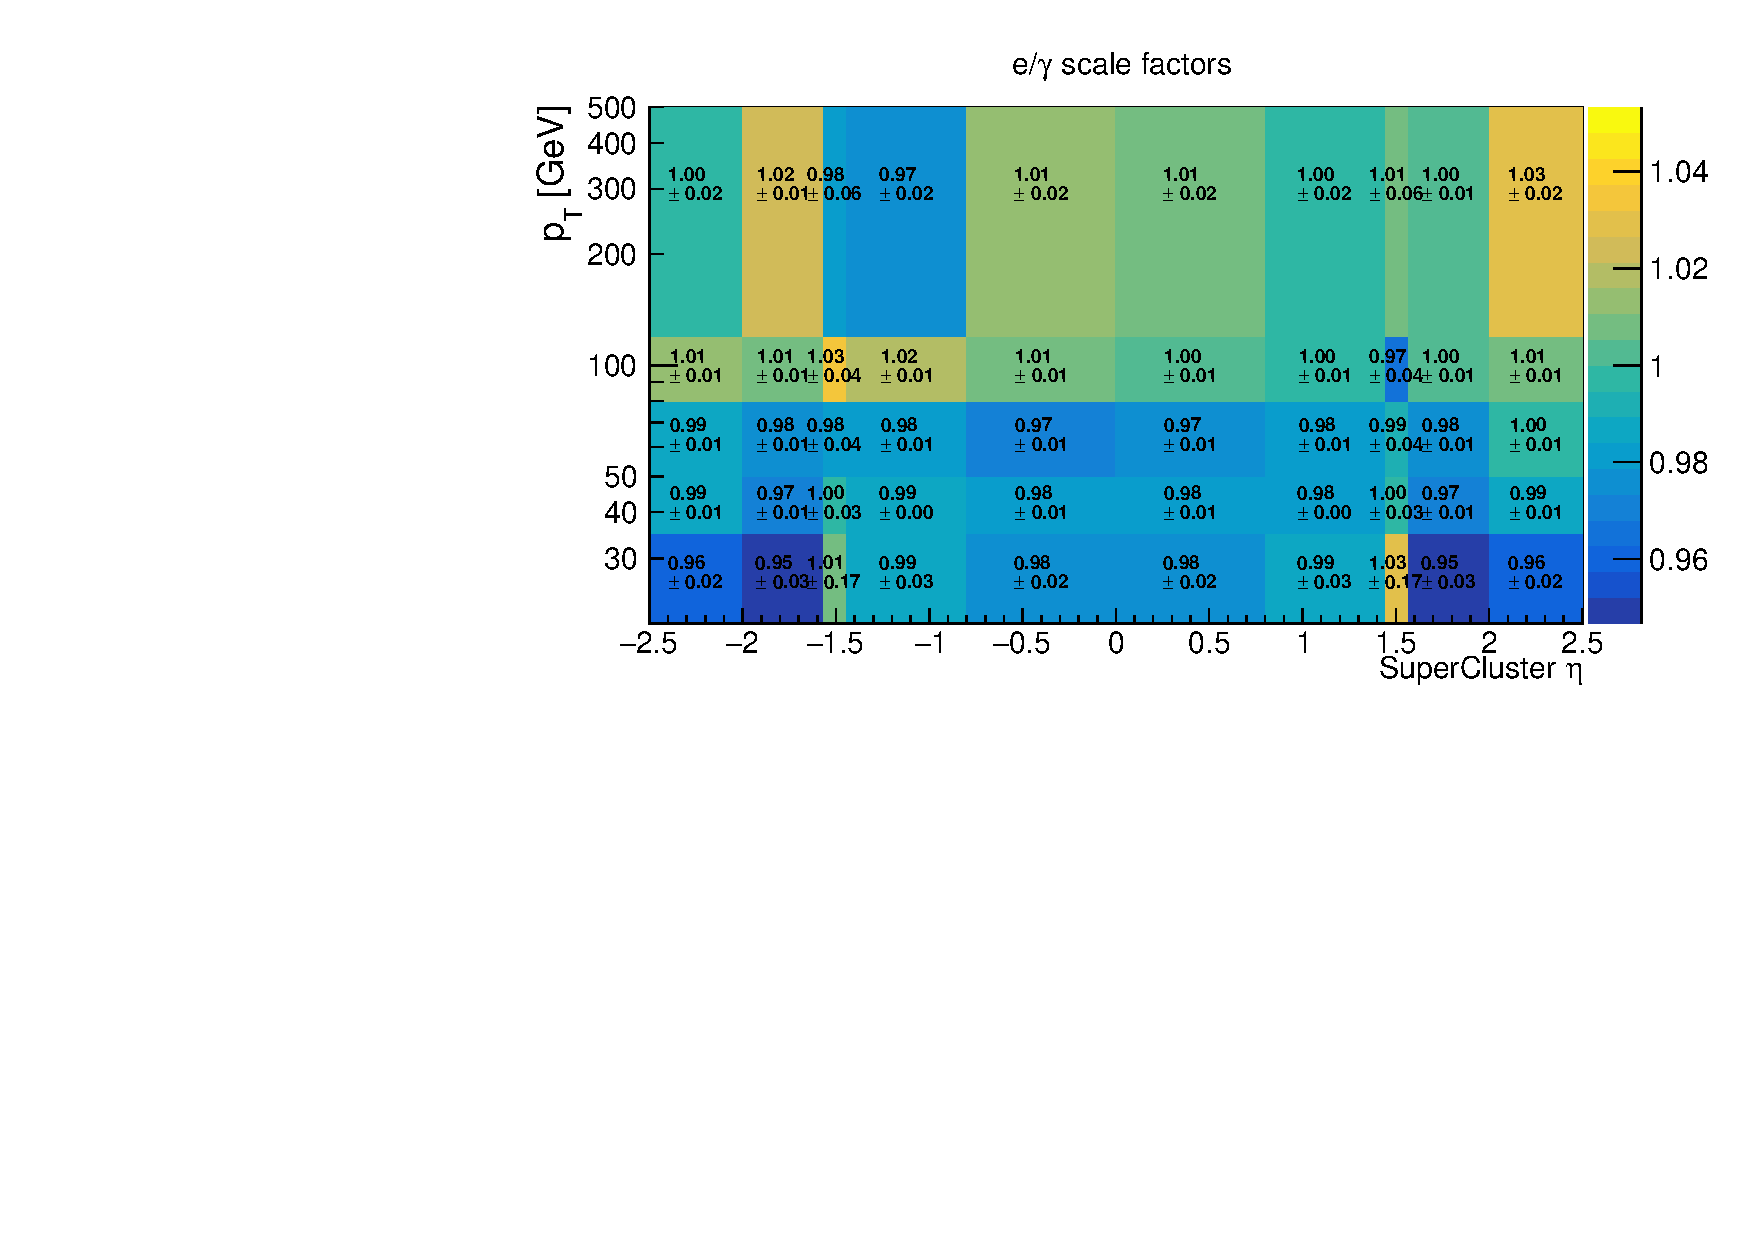
\includegraphics[width=.5\textwidth]{SF/phEffSF_2016postVFP.pdf}}}\\
\subfigure [2017]        {\resizebox{.5\textwidth}{!}{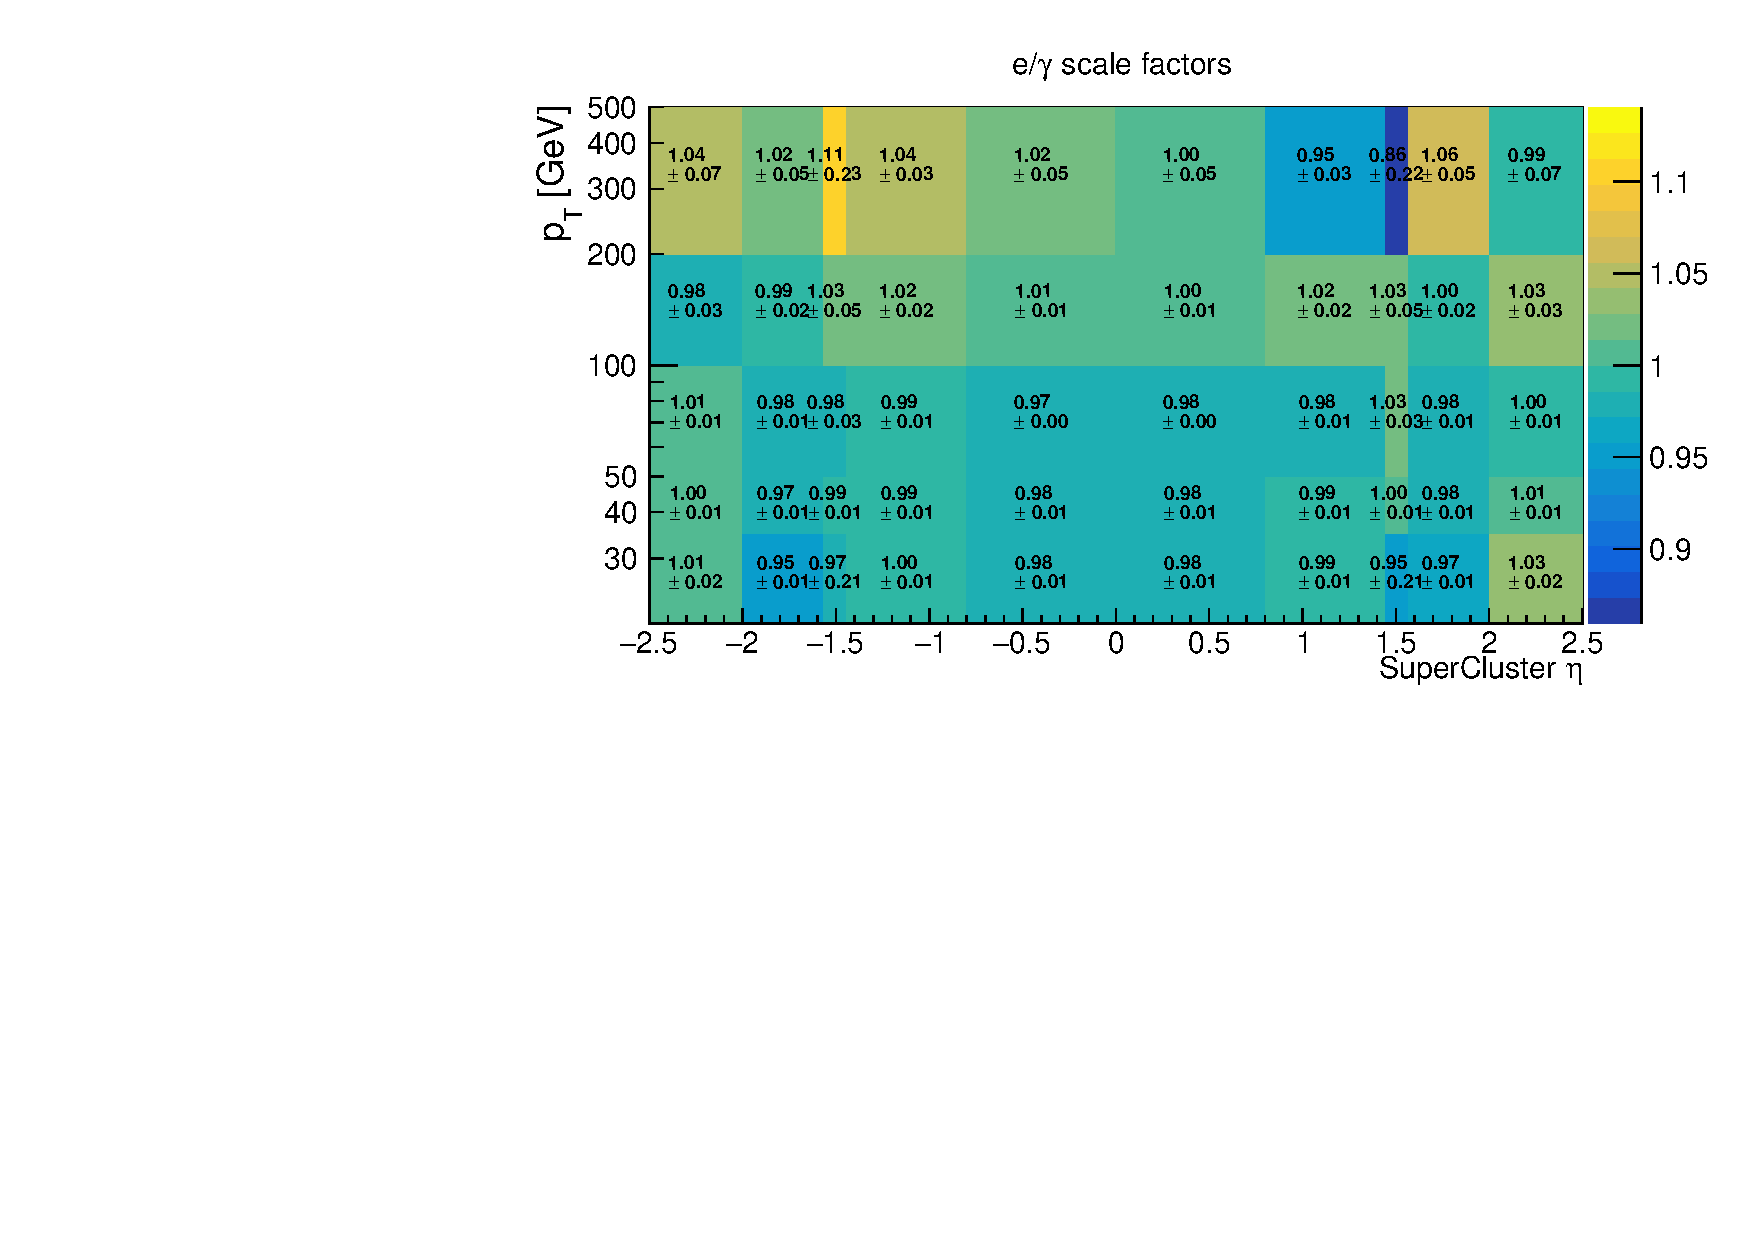
\includegraphics[width=.5\textwidth]{SF/phEffSF_2017.pdf}}}
\subfigure [2018]        {\resizebox{.5\textwidth}{!}{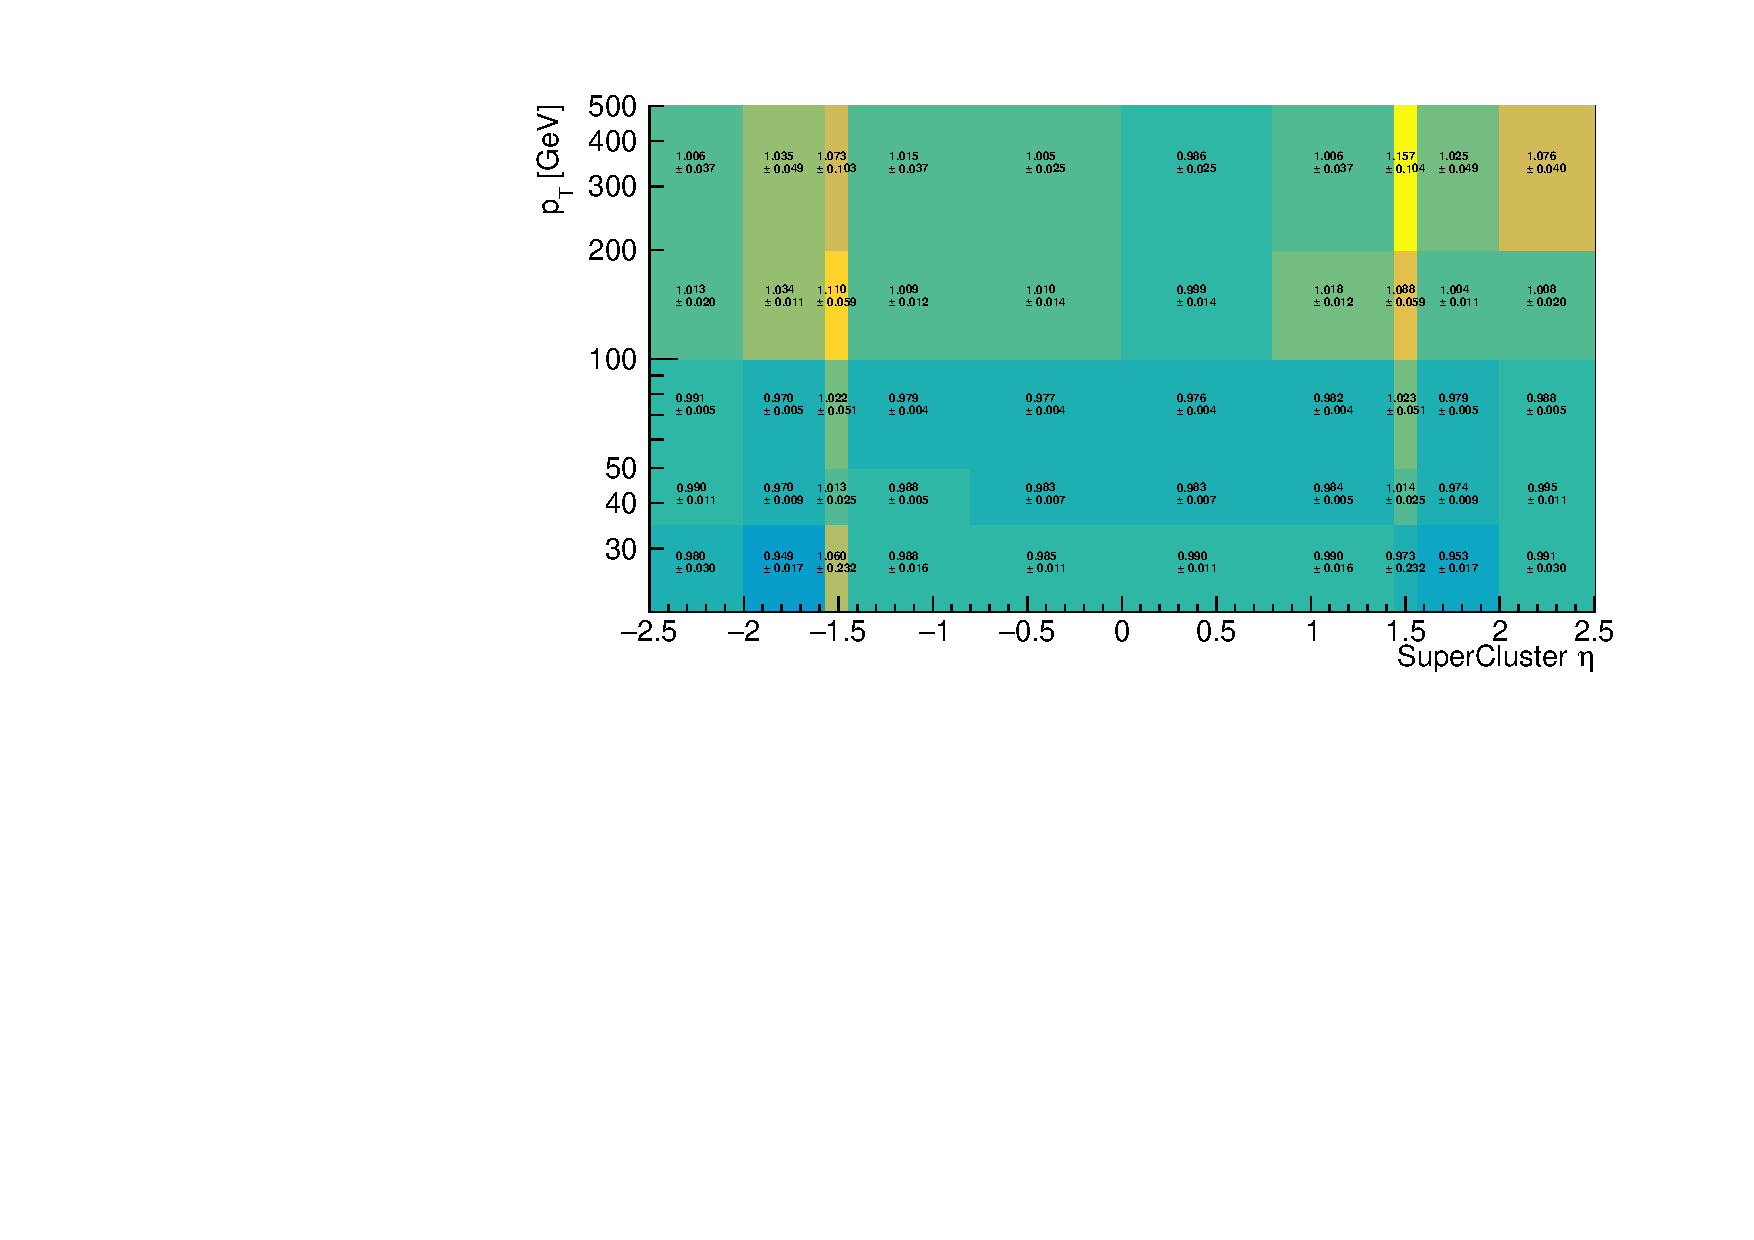
\includegraphics[width=.5\textwidth]{SF/phEffSF_2018.pdf}}}
\caption{Photon efficiency scale factors for the POG cut-based Loose ID.}
\label{fig:phEffSF}
\end{figure}

Besides the identification working points, an electron veto selection (CSEV veto) is also applied.
%% The scale factors are shown in ~\ref{tab:eleveto_SFs}.

%% \begin{table}[htbp]
%%  \centering
%%    \begin{tabular}{|c|c|l|l|}
%%    \hline
%%    Year & $p_T$& barrel & endcap\\ \hline
%%    2016 & inclusive &0.9938 $\pm$ 0.0119 & 0.9875 $\pm$ 0.0044\\\hline
%%    2017 & inclusive & 0.9862 $\pm$ 0.0030 & 0.9638 $\pm$ 0.0047\\\hline
%%    \multirow{3}{*}{2018} &10 GeV$<p_{T}^{\gamma}<30$ GeV &0.9869 $\pm$ 0.0043& 0.9535 $\pm$ 0.0054\\
%%    & 30 GeV$<p_{T}^{\gamma}<$60 GeV  &0.9908  $\pm$ 0.0111 & 0.9646 $\pm$ 0.0076\\
%%    & 60 GeV$<p_{T}^{\gamma}<$200 GeV &1.0084  $\pm$ 0.0856& 1.0218 $\pm$ 0.1178\\
%%    \hline
%%    \end{tabular}
%%    \caption{Electron veto scale factors for barrel and endcap corresponding to 2016 to 2018.}
%%    \label{tab:eleveto_SFs}
%%  \end{table}

%\begin{figure}[b]
%  \begin{center}
%    \includegraphics[width=0.8\textwidth]{figs/photon_SFs.pdf}
%    \caption{Photon ID scale factors for cut-based loose Photon selection}
%    \label{fig:PhotonEff}
%  \end{center}
%\end{figure}

\paragraph{Multivariate ID}
The multivariate (MVA) ID employs 14 variables linked to the energy and shower shape of the ECAL supercluster associated with the photon, as well as its isolation from other particles in the event.
These variables include those utilised by the cut-based ID, so the two are not independent.
The full list is shown in Table \ref{tab:MVAvariables}.
The version used is \texttt{RunIIFall17v2}.

\begin{table}[ht]
\caption[.]{Variables used by the MVA-based ID, version \texttt{RunIIFall17v2}}
\label{tab:MVAvariables}
\centering
\begin{tabular}{l|l}
Name & variable\\
\hline
SCRawE             & superCluster.rawEnergy                                               \\
r9                 & r9                                                                   \\
sigmaIetaIeta      & full5x5\_showerShapeVariables.sigmaIetaIeta                          \\
etaWidth           & superCluster.etaWidth                                                \\
phiWidth           & superCluster.phiWidth                                                \\
covIEtaIPhi        & full5x5\_showerShapeVariables.sigmaIetaIphi                          \\
s4                 & full5x5\_showerShapeVariables.e2x2/full5x5\_showerShapeVariables.e5x5\\
scEta              & superCluster.eta                                                     \\
rho                & fixedGridRhoAll                                                      \\
esEffSigmaRR       & full5x5\_showerShapeVariables.effSigmaRR                             \\
esEnergyOverRawE   & superCluster.preshowerEnergy/superCluster.rawEnergy                  \\
phoIso03           & photonIso                                                            \\
chgIsoWrtChosenVtx & chargedHadronIso                                                     \\
chgIsoWrtWorstVtx  & chargedHadronWorstVtxIso                                             \\
\end{tabular}
\end{table}

Two working points are provided centrally by the EGamma POG: \texttt{wp90} and \texttt{wp80}, corresponding to 90 \% and 80 \% prompt photon efficiency respectively.
The cuts on the MVA estimator value that define the two working points are detailed in Table \ref{tab:MVAwpCuts}.

\begin{table}[ht]
\caption[.]{Working points of the photon MVA-based ID, version \texttt{RunIIFall17v2}}
\label{tab:MVAwpCuts}
\centering
\begin{tabular}{|l|c|c|}
\hline
Name & Barrel & Endcap \\
\hline
\texttt{wp80} & -0.02 & -0.26 \\
\texttt{wp90} &  0.42 &  0.14 \\
\hline
\end{tabular}
\end{table}

\begin{figure}
\begin{center}
\subfigure [2016preVFP ] {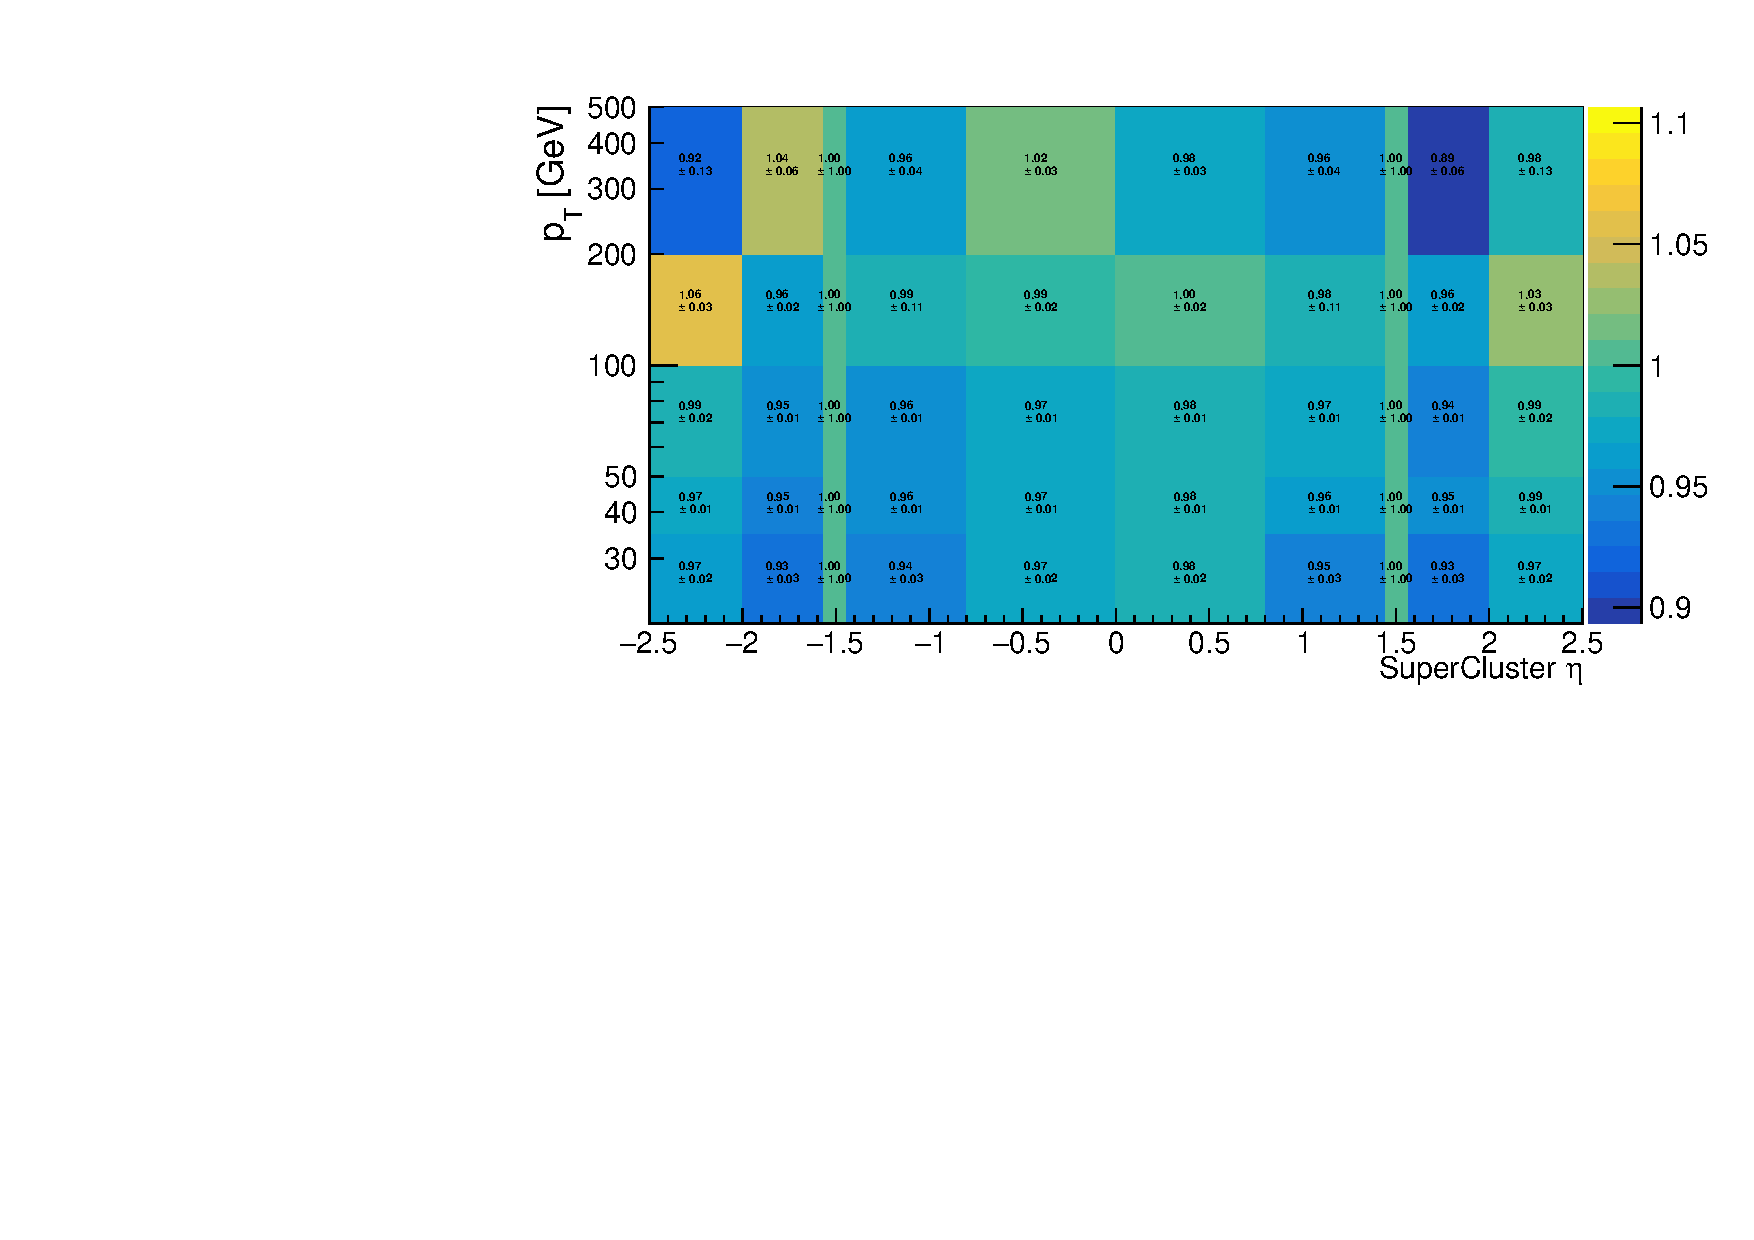
\includegraphics[width=.5\textwidth]{SF/2016_PhotonsMVAwp80_SF2D.pdf}}%
\subfigure [2017]        {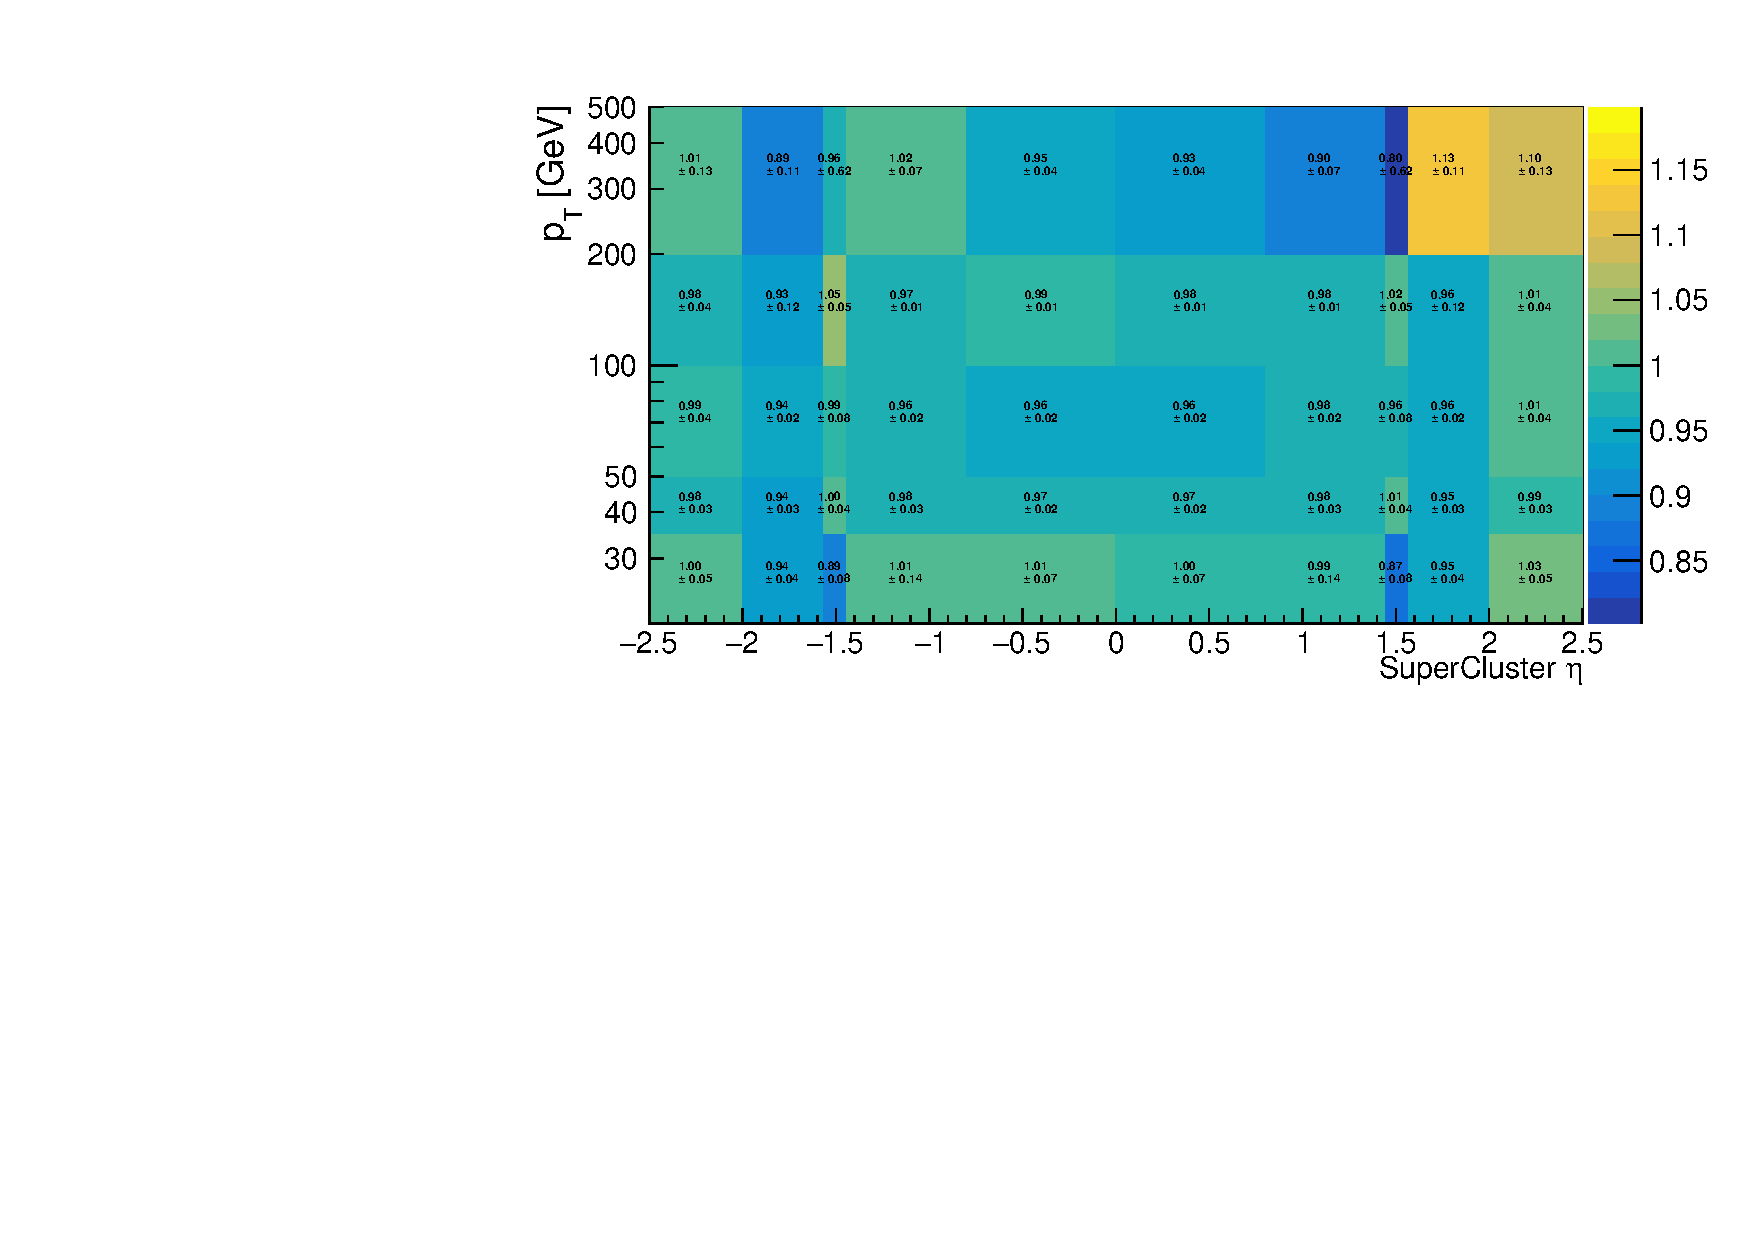
\includegraphics[width=.5\textwidth]{SF/2017_PhotonsMVAwp80_SF2D.pdf}}\\
\subfigure [2018]        {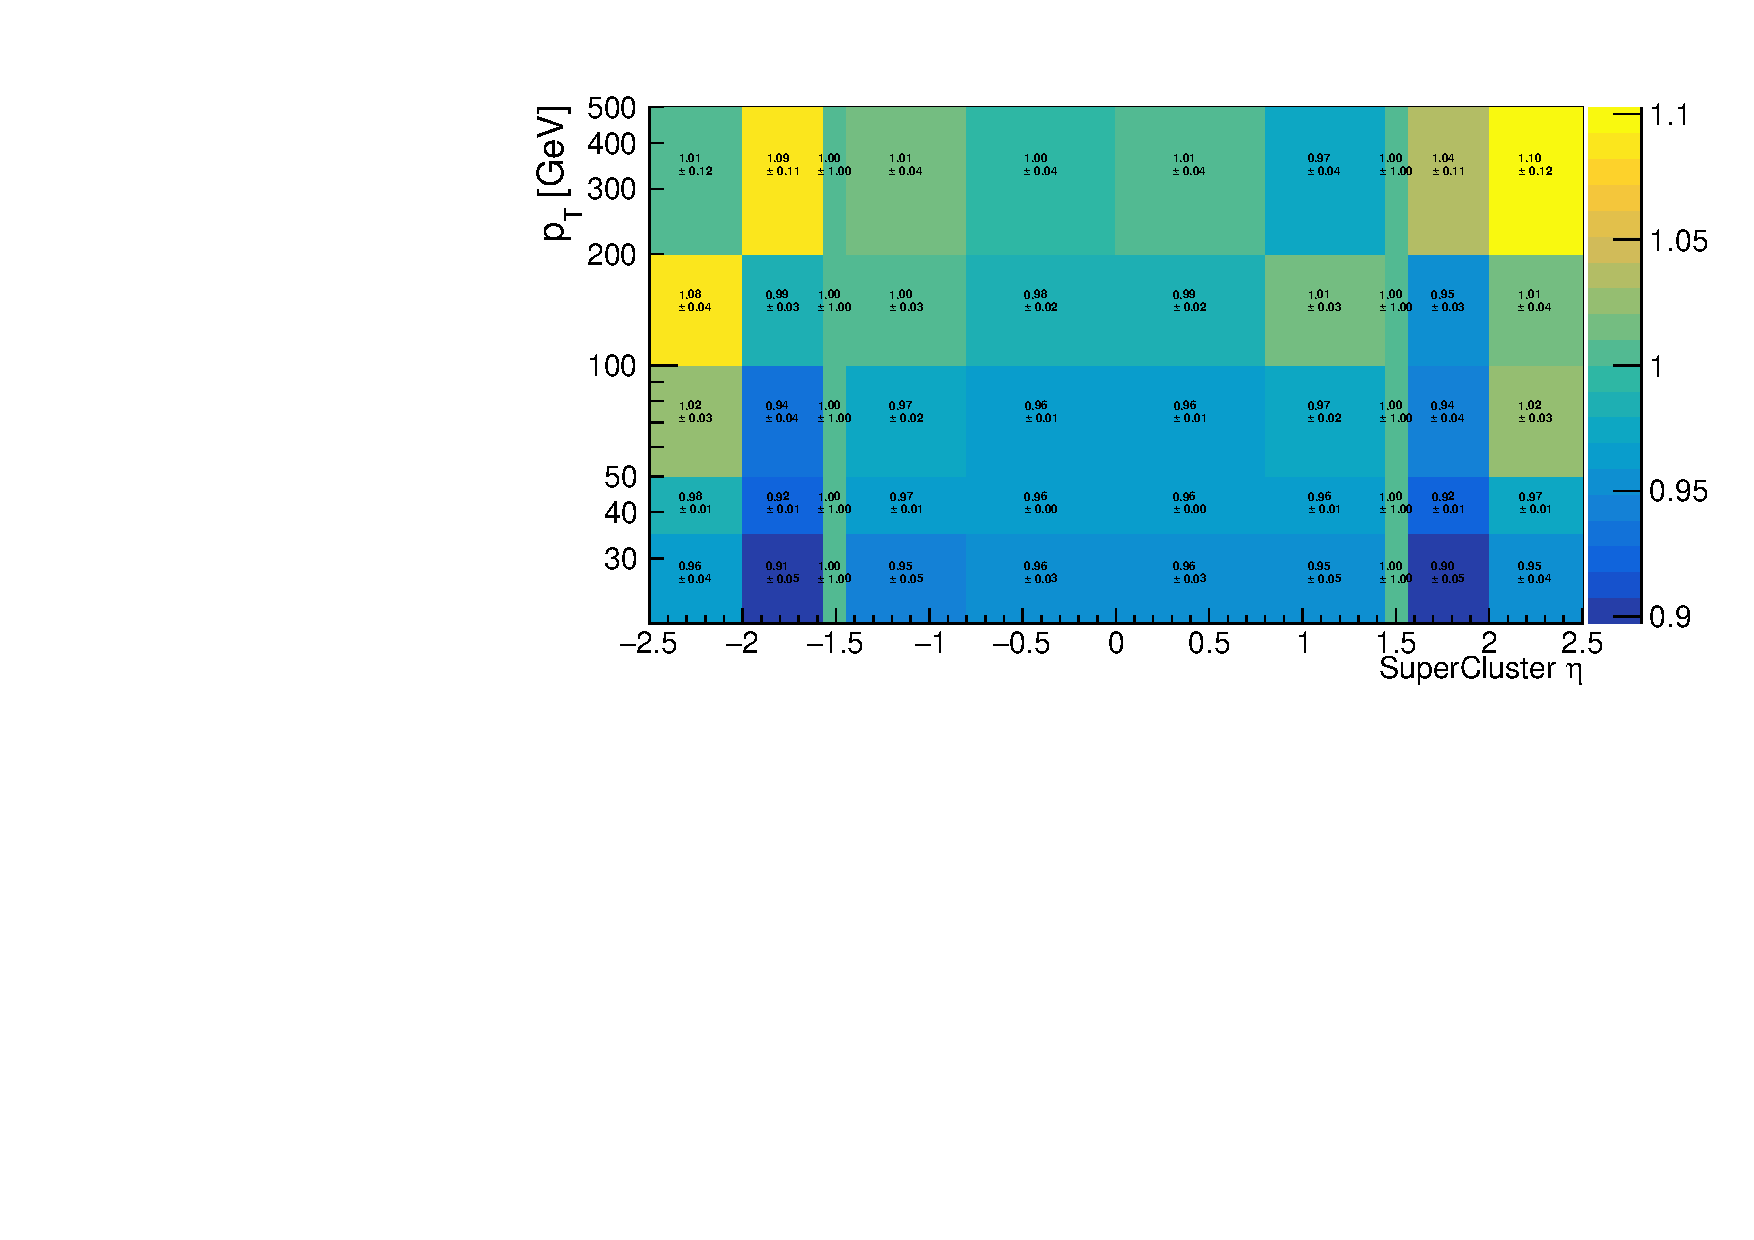
\includegraphics[width=.5\textwidth]{SF/2018_PhotonsMVAwp80_SF2D.pdf}}
\end{center}
\caption{Photon efficiency scale factors for the POG MVA-based ID with working point \texttt{wp80}.}
\label{fig:phEffMVASF_wp80}
\end{figure}

\begin{figure}
\centering
\subfigure [2016preVFP ] {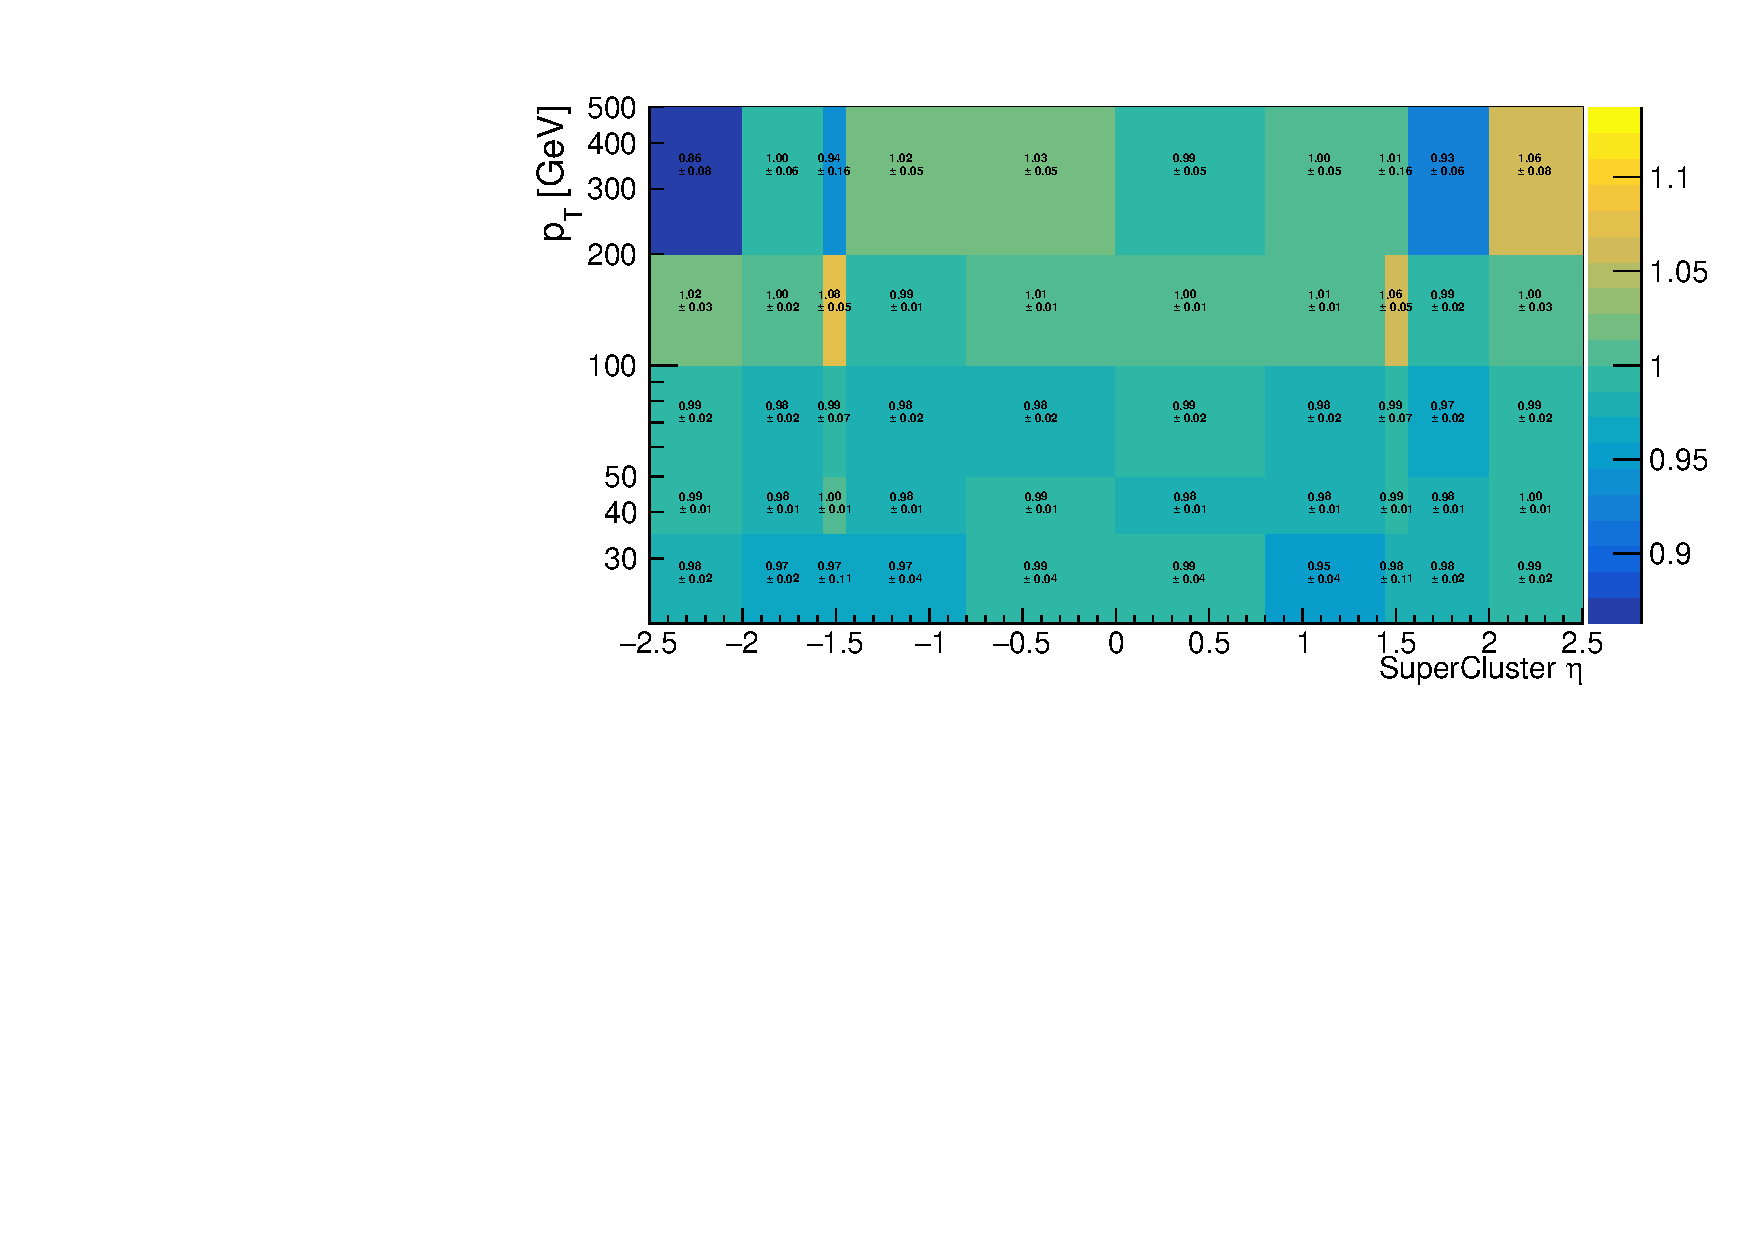
\includegraphics[width=.5\textwidth]{SF/2016_PhotonsMVAwp90_SF2D.pdf}}%
\subfigure [2017]        {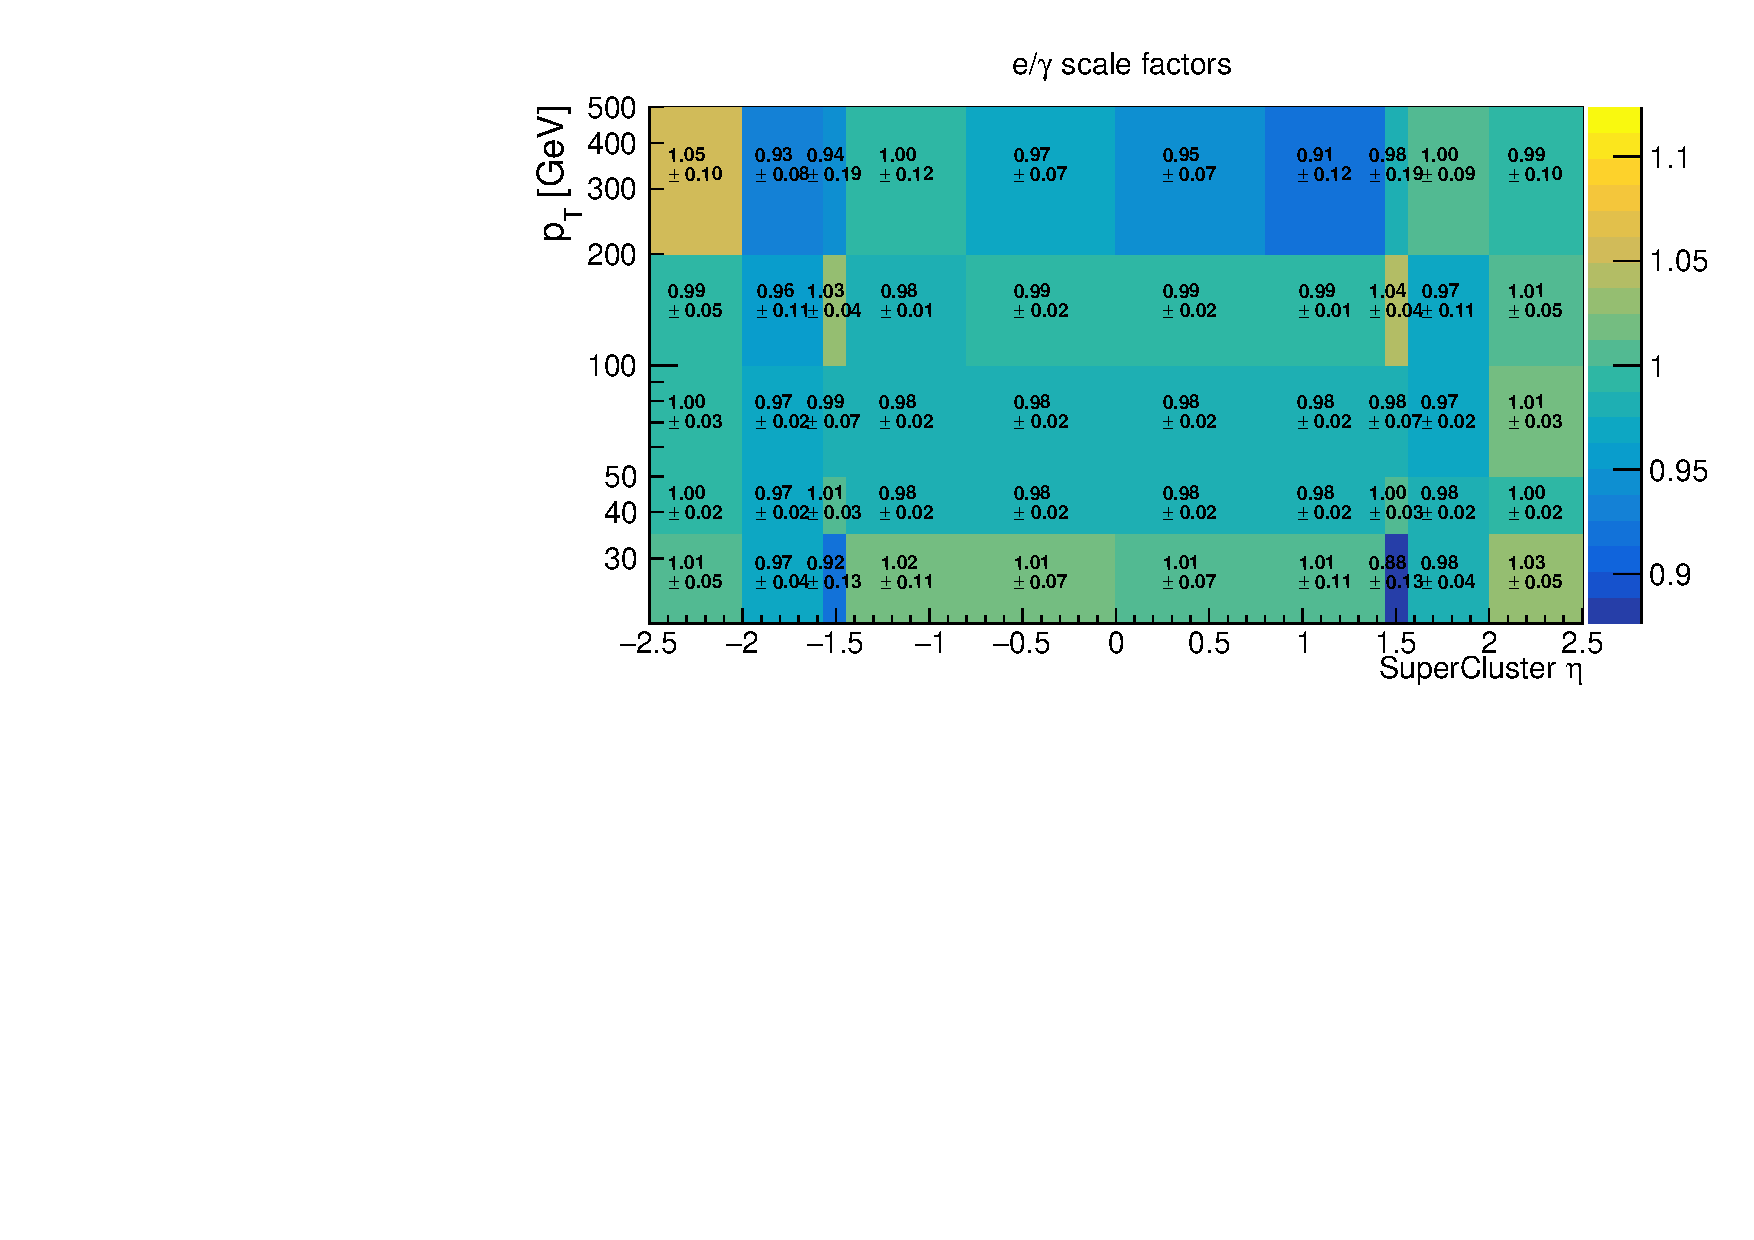
\includegraphics[width=.5\textwidth]{SF/2017_PhotonsMVAwp90_SF2D.pdf}}\\
\subfigure [2018]        {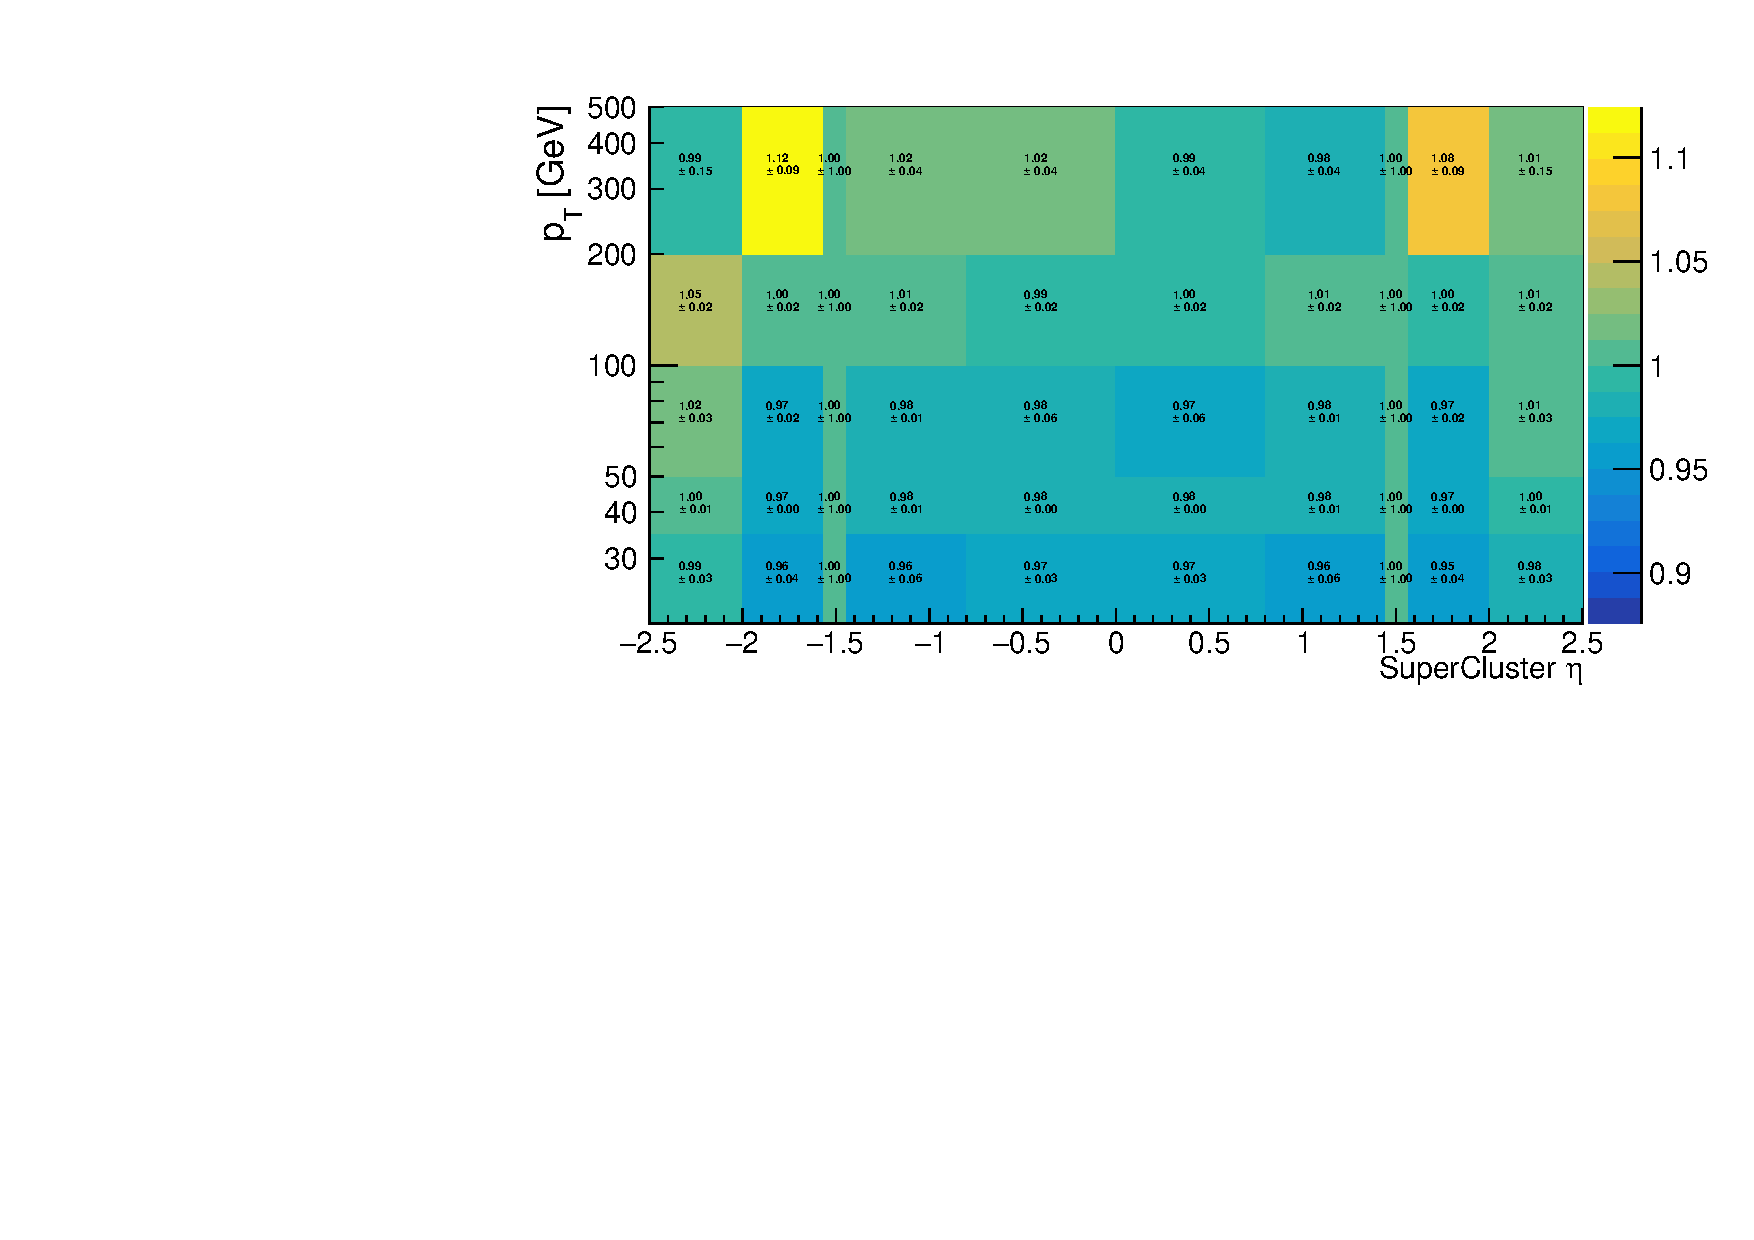
\includegraphics[width=.5\textwidth]{SF/2018_PhotonsMVAwp90_SF2D.pdf}}
\caption{Photon efficiency scale factors for the POG MVA-based ID with working point \texttt{wp90}.}
\label{fig:phEffMVASF_wp90}
\end{figure}
